So for the business process, as stated previously, we have a set of activities that organizes the trucks and their drivers.
In the goal of have their workflow optimized.

And it goes as follows:

\begin{center}
    \includegraphics[width=1\textwidth]{images/flowchart}
\end{center}

To give more context to the diagram above, we will dive into the details of it processes.

So first of all we have the following core processes:

\begin{itemize}
    \item Welcome of the driver
    \item Digitalization of documents
    \item Secure access to logistics platform
    \item Dashboard for the management
\end{itemize}

Starting by welcoming the driver, this process relies on the driver to introduce himself, his credentials,
scan any documents related to the transportation and also have a signature of the driver for the legal purposes
all that present at a kiosk, once all that data has been input the driver is invited to wait at the truck awaiting
the response from the management.

Then there is the digitalization of the documents which is the process of the driver to have a digital copy
of the documents that are all sent to the management dashboard for verification and approval, to give sign
to the driver that the documents are correct and that he can proceed to the next step, sending the approval
is done through sending a notification either through the phone application, an sms or calling by pager.

Next comes the secure access to the logistics platform, this process is mainly related to infrastructure gate,
the driver has a special access code to the platform, this code is generated by the management and is sent to
the driver by sms or through the application, once the driver accesses the platform the management is notified
by his arrival.

Finally, the dashboard for the management is the main interface for the management and it's divided into multiple
workspaces depending on the role and priveledges of the user depending on the needs of the clients.

As of the current time, the application is as follows:

\begin{center}
    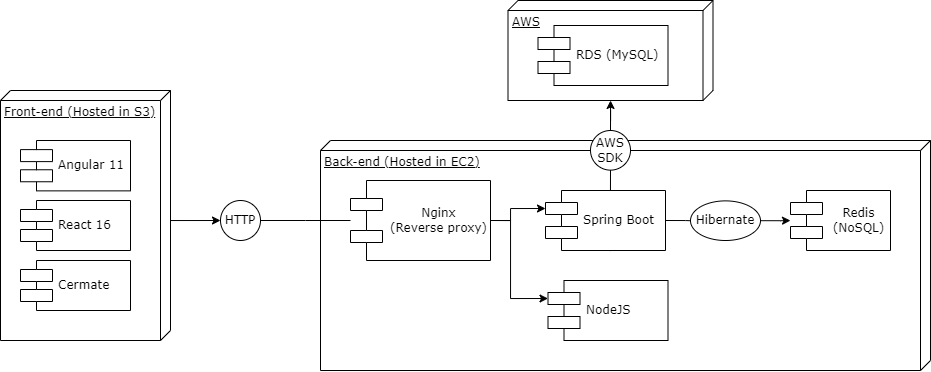
\includegraphics[width=0.8\textwidth]{images/State-of-art}
\end{center}

So it's built with different technologies for the front depending on the platform or device
that is handling it, and for the backend it's handled mainly in Spring and NodeJs, for
the database it's handled for the realtime data with Redis, and for the user data it's 
handled in RDS MySQL database, for everything that is related to handling notifications
it's done through the MQTT broker and Google Firebase service.

The Spring application is handling everything from the user data, managemenet of the sites,
the trucks and drivers, the geolocalisation, the notification mapping, the realtime data
handling.

